\lecture{3}{1. September 2025}{Control volume analysis I: Basic laws and mass conservation}

\exercise{4.5}
A \qty{0,3}{m} by \qty{0,5}{m} rectangular air duct carries a flow of \qty{0,45}{m^3/s} at a density of \qty{2}{kg/m^3}, Calculate the mean velocity in the duct. If the duct tapers to \qty{0,15}{m} by \qty{0,5}{m} size, determine the mean velocity in this section if the density is \qty{1,5}{kg/m^3} in this section.
\bigbreak
In the initial state \qty{0,45}{m^3/s} of air is passing by an area \qty{0,3}{m} by \qty{0,5}{m}. This area is:
\[ 
A = \qty{0,3}{m} \cdot \qty{0,5}{m} = \qty{0,15}{m^2} 
.\]
Now if we divide the flow by the area through which it passes we will obtain the velocity of the air as:
\[ 
V_1 = \frac{\qty{0,45}{\frac{m^3}{s}} }{\qty{0,15}{m^2} } = \qty{3}{\frac{m}{s}} 
.\]
Therefore the air will initially be moving at a velocity of $V_1 = \qty{3}{\frac{m}{s}}$. 

As mass if a conserved property the mass flow in the initial section must equal the mass flow of the tapered section. Using the continuity equation we can calculate the mass flow rate initially as:
\[ 
\dot{m}_1 = \rho_1 V_1 A_1 = \qty{2}{\frac{kg}{m^3}} \cdot \qty{3}{\frac{m}{s}} \cdot \qty{0,15}{m^2} = \qty{0,9}{\frac{kg}{s}}
.\]
This must equal the mass flow rate after the taper, thus:
\begin{align*}
  \dot{m}_1 &= \dot{m}_2 \\
  \dot{m}_1 &= \rho_2 V_2 A_2 \\
  V_2 &= \frac{\dot{m}_1}{\rho_2 A_2} \\
  V_2 &= \frac{\qty{0,9}{\frac{kg}{s}} }{\qty{1,5}{\frac{kg}{m^3}} \cdot \qty{0,15}{m} \cdot \qty{0,5}{m}} \\
  V_2 &= \qty{8}{\frac{m}{s}} 
.\end{align*}
Therefore the mean velocity of the tapered section is \qty{8}{m/s}. 


\exercise{4.9}
A pipeline \qty{0,3}{m} in diameter divides at a $Y$ into two branches \qty{200}{mm} and \qty{150}{mm} in diameter. If the flow rate in the main line is \qty{0,3}{m^3/s} and the mean velocity in the \qty{200}{mm} pipe is \qty{2,5}{m/s}, determine the flow rate in the \qty{150}{mm} pipe.
\bigbreak
We assume that the water flow can be modelled as steady and incompressible through a fixed control volume. In this case the continuity equation simplifies to:
\[ 
\int_{\mathrm{CS}} \textbf{V} \cdot \mathrm{d}\textbf{A} = 0
\]
or
\[ 
V_1 A_1 = V_2 A_2 + V_3 A_3
.\]
Using the flow rates $Q_1 = V_1 A_1$, $Q_2 = V_2 A_2$, and $Q_3 = V_3 A_3$ we can write:
\[ 
Q_1 = Q_2 + Q_3
.\]
Let the \qty{150}{mm} pipe be number 3 and we can then isolate the flow rate we wish to find $Q_3$ in this as:
\[ 
Q_3 = Q_1 - Q_2
.\]
We can now find the flow rate of $Q_2$ as
\[ 
Q_2 = V_2 A_2 = \qty{2,5}{\frac{m}{s}} \cdot \pi \cdot \left( \qty{100}{mm}  \right)^2 = \qty{0,0785}{\frac{m^3}{s}} 
.\]
And thus the flow rate in the \qty{150}{mm} pipe $Q_3$ can be found as:
\[ 
Q_3 = \qty{0,3}{\frac{m^3}{s}} - \qty{0,0785}{\frac{m^3}{s}} = \qty{0,221}{\frac{m^3}{s}} 
.\]


\exercise{4.12}
A cylindrical tank, of diameter $D = \qty{150}{mm}$, drains through an opening, $d = \qty{5}{mm}$, in the bottom of the tank. The speed of the liquid leaving the tank is approximately $V = \sqrt{2gy}$, where $y$ is the height from the tank bottom to the free surface. If the tank is initially filled with water to $y_0 = \qty{0,4}{m}$, determine the water depths at $t = \qty{60}{s}$, $t = \qty{120}{s}$, and $t = \qty{180}{s}$. Plot $y(m)$ versus $t$ for the first \qty{180}{s}.
\bigbreak
We assume uniform incompressible flow. The continuity equation states:
\[ 
\frac{\partial}{\partial t} \int_{\mathrm{CV}} \rho \, \mathrm{d}V + \int_{\mathrm{CS}} \rho \textbf{V} \cdot \mathrm{d}\textbf{A} = 0
.\]
In other words, the rate increase of mass in the control volume plus the mass outflow from the control volume equals zero. If we treat the tank as out control volume we get:
\begin{align*}
  \frac{\partial }{\partial t} \int_{0}^{y} \rho \cdot A_{\mathrm{tank}} \, \mathrm{d}y + \rho \cdot V \cdot A_{\mathrm{opening}} &= 0 \\
  \rho \cdot \pi \cdot R^2 \cdot \frac{\mathrm{d}y}{\mathrm{d}t} + \rho \cdot \pi \cdot r^2 \cdot V &= 0
.\end{align*}
We can now use $V = \sqrt{2gy}$ and get:
\begin{align*}
  \rho \cdot \pi \cdot R^2 \cdot \frac{\mathrm{d}y}{\mathrm{d}t} + \rho \cdot \pi \cdot r^2 \cdot \sqrt{2gy} &= 0 \\
  R^2 \, \frac{\mathrm{d}y}{\mathrm{d}t} + r^2 \cdot \sqrt{2gy} &= 0 \\
  \frac{\mathrm{d}y}{\mathrm{d}t} &= - \frac{r^2}{R^2} \cdot \sqrt{2gy}
.\end{align*}
Separating variables we get:
\[ 
\frac{1}{y^{\frac{1}{2}}} \, \mathrm{d}y = - \frac{r^2}{R^2} \cdot \sqrt{2g} \, \mathrm{d}t
.\]
Integrating we get:
\begin{align*}
  2 \left( y^{\frac{1}{2}} - y_0^{\frac{1}{2}} \right) &= - \frac{r^2}{R^2} \sqrt{2g}t \\
  y^{\frac{1}{2}} &= - \frac{r^2}{R^2} \sqrt{\frac{g}{2}} t + y_0^{\frac{1}{2}} \\
  y^{\frac{1}{2}} &= y_0^{\frac{1}{2}} \left( 1 - \frac{r^2}{R^2} \sqrt{\frac{g}{2y_0}} t \right) \\
  y &= y_0 \left( 1 - \left( \frac{r}{R} \right)^2 \sqrt{\frac{g}{2 y_0}} t \right)^2
.\end{align*}
We have that $y_0 = \qty{0,4}{m}$ and $\frac{r}{R} = \frac{\qty{2,5}{mm}}{\qty{75}{mm}} = \frac{1}{30}$. At $t = \qty{60}{s}$ we therefore get:
\[ 
  y_{\qty{60}{s}} = \qty{0,4}{m} \cdot \left( 1 - \left( \frac{1}{30} \right)^2 \sqrt{\frac{\qty{9,81}{\frac{m}{s^2}}}{2 \cdot \qty{0,4}{m}}} \cdot \qty{60}{s}  \right)^2 = \qty{0.235}{m}
.\]
At $t = \qty{120}{s}$ we get
\[ 
y_{\qty{120}{s}} = \qty{0,4}{m} \cdot \left( 1 - \left( \frac{1}{30} \right)^2 \sqrt{\frac{\qty{9,81}{\frac{m}{s^2}}}{2 \cdot \qty{0,4}{m}}} \cdot \qty{120}{s}  \right)^2 = \qty{0,114}{m}
.\]
And at $t = \qty{180}{s}$ we get:
\[ 
y_{\qty{180}{s}} = \qty{0,4}{m} \cdot \left( 1 - \left( \frac{1}{30} \right)^2 \sqrt{\frac{\qty{9,81}{\frac{m}{s^2}}}{2 \cdot \qty{0,4}{m}}} \cdot \qty{180}{s}  \right)^2 = \qty{0,036}{m}
.\]
$y(m)$ versus $t$ has been plotted in GeoGebra on \autoref{fig:e4_12}

\begin{figure} [ht]
  \centering
  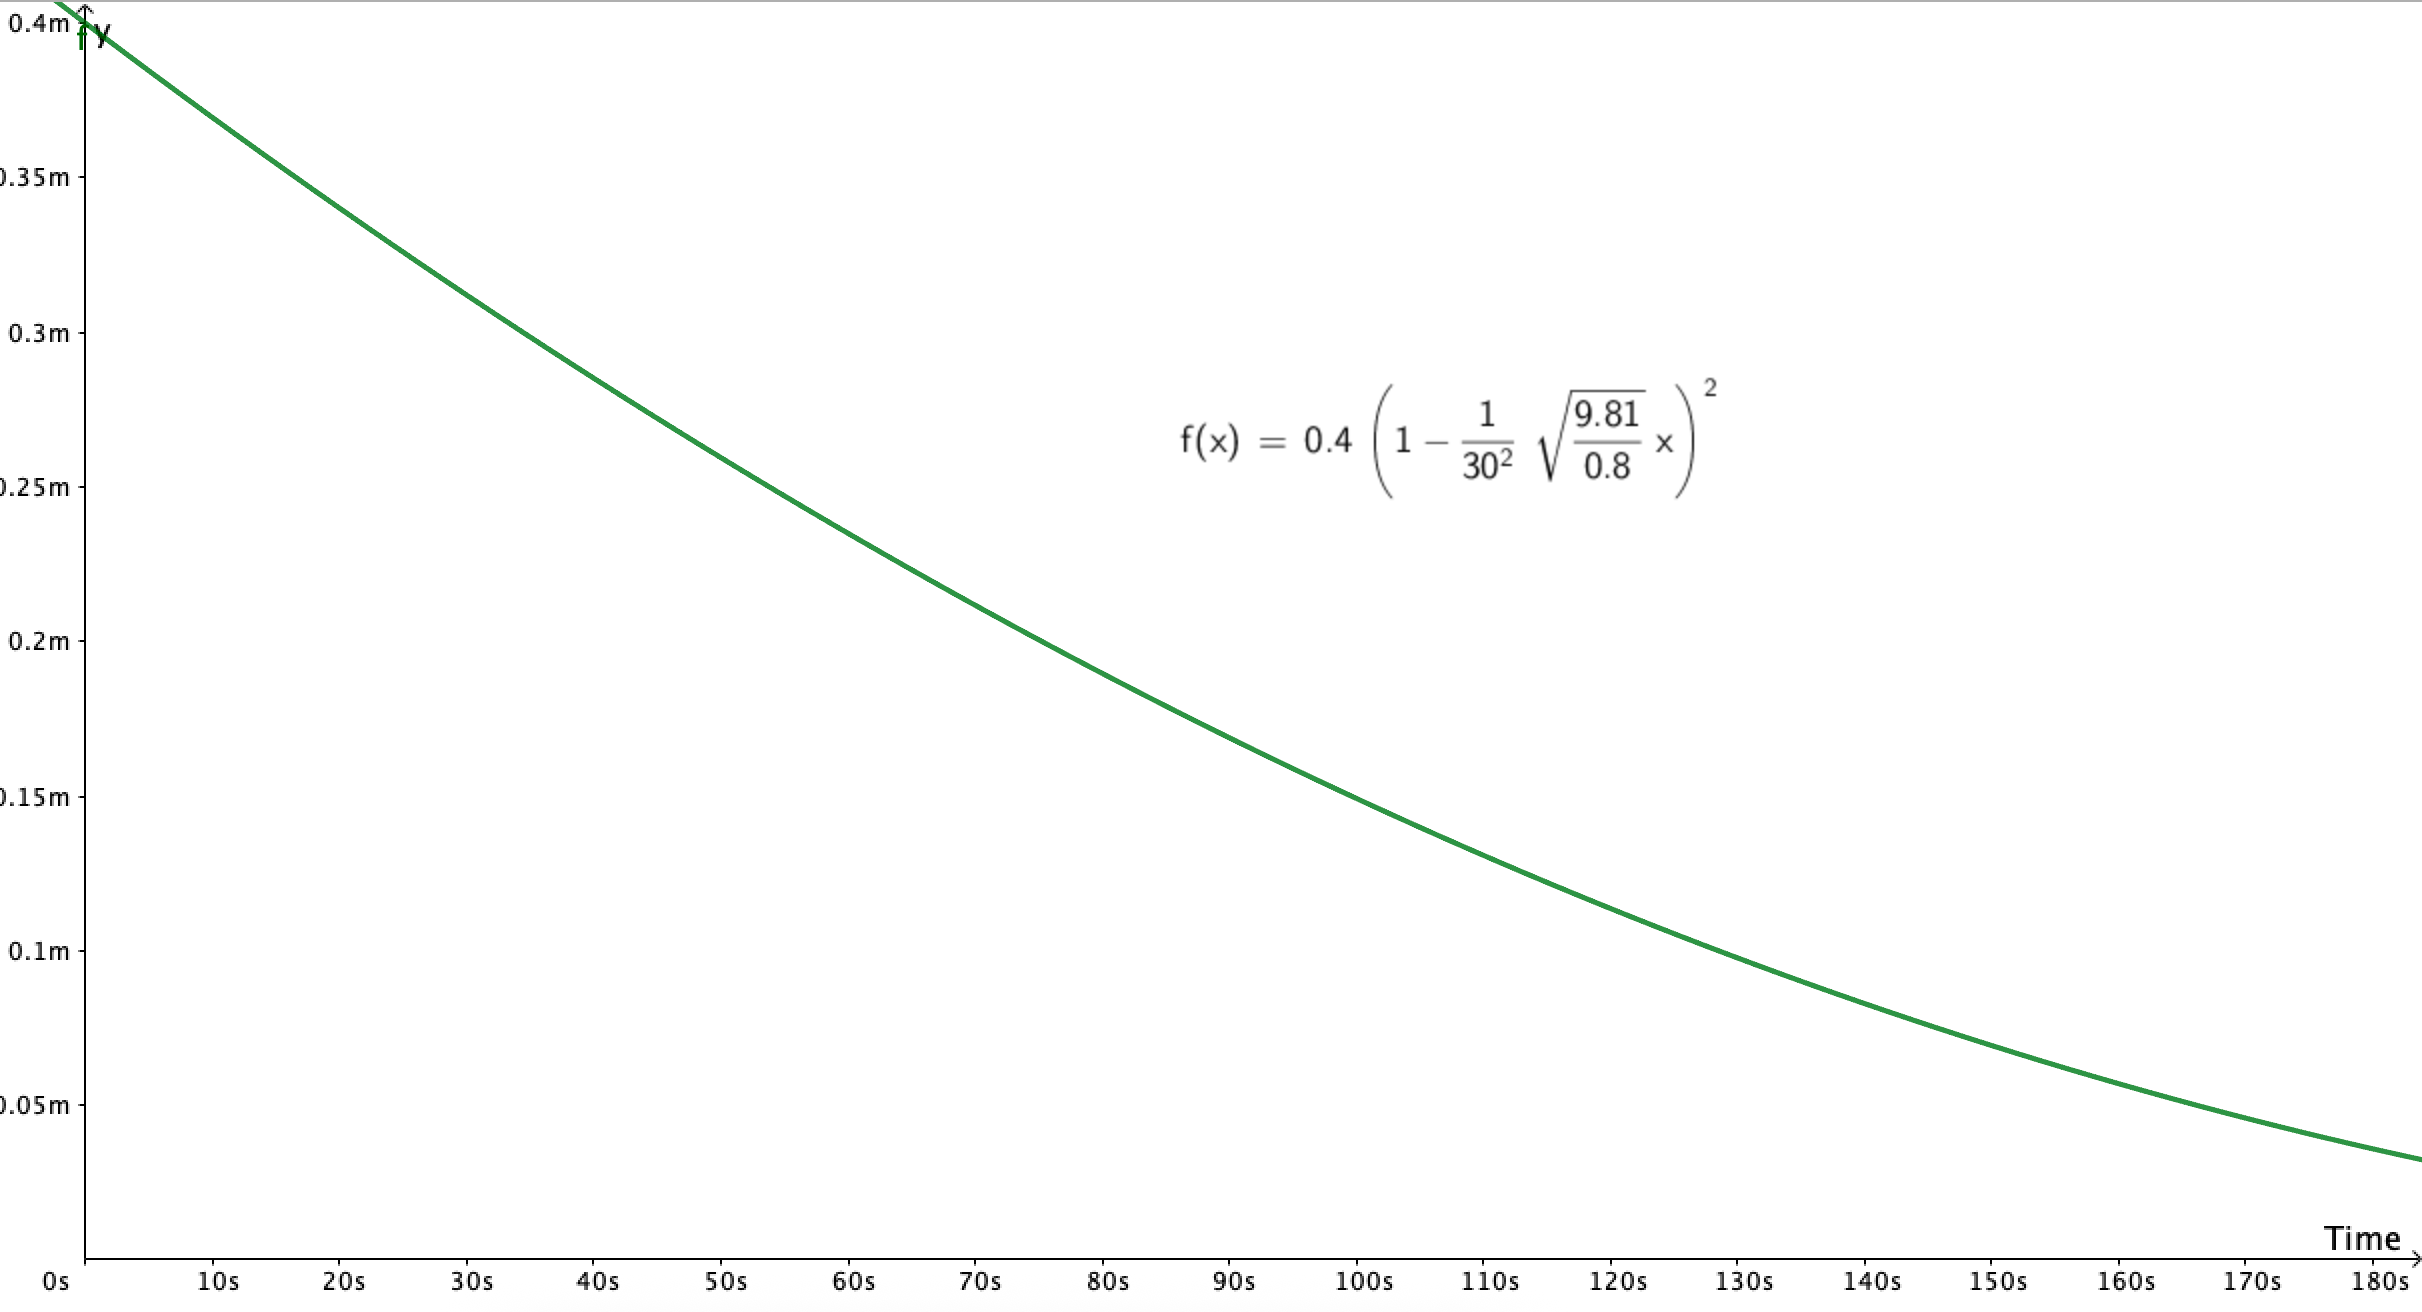
\includegraphics[width=0.8\linewidth]{./figures/e4_12.png}
  \caption{Plot of $y(m)$ versus $t$.}
  \label{fig:e4_12}
\end{figure}
